\chapter{Background and Related Work}
\label{chap:background}

% The goal of this chapter is for laying the technical background (such as distributed source coding) for understanding the contribution of your thesis; non-technical background (such as the background of M2M communications) can go to Chapter~\ref{chap:introduction}.

% Related work should be be classified into proper sub-sections depending on the topics
% related to your thesis research.
\section{Random Access Procedure}
The random access procedure in 5G is a critical mechanism that allows a User Equipment (UE) to establish initial uplink synchronization and connect to the network (gNB). The procedure is essential for first-time access, handovers, and re-establishing connections after inactivity or loss of synchronization. Here are some typical steps in contention-based random access: 
\begin{itemize}
    \item Preamble Transmission (Msg1): The UE randomly selects a PRACH (Physical Random Access Channel) preamble and transmits it to the gNB. This "signature" indicates the UE's request for network access.

    \item Random Access Response (Msg2): The gNB detects the preamble and responds with a Random Access Response (RAR), which includes timing adjustment, a temporary identity, and an uplink resource grant. This enables the UE to align its timing with the network and prepare for further communication.

    \item RRC Connection Request (Msg3): Using the granted resources, the UE sends a connection request, which includes its identity and the reason for establishing the connection, such as initial access or handover.

    \item Contention Resolution (Msg4): The gNB sends a contention resolution message confirming which UE has successfully completed the random access. If multiple UEs used the same preamble, only the correct one will be acknowledged, resolving the contention.
\end{itemize}

\section{Synchronization Signal Block}
\subsection{Components of SSB}
The Synchronization Signal Block (SSB) in 5G New Radio (NR) is a critical structure for initial access between the user equipment (UE) and the base station (gNB). Each SSB is composed of three main elements:
\begin{itemize}
    \item Primary Synchronization Signal (PSS): The PSS enables the UE to obtain symbol timing and perform coarse frequency synchronization. It allows the UE to find the starting point of a radio frame and resolves the physical layer cell identity group.
    \item Secondary Synchronization Signal (SSS): The SSS complements PSS by providing additional information to finalize the cell identification and determines the frame timing, which refines synchronization accuracy for the UE.
    \item Physical Broadcast Channel (PBCH): The PBCH conveys essential cell-specific information, including system configuration parameters (such as the System Frame Number), which the UE needs for further connection setup after synchronization.
\end{itemize}
These components jointly allow the UE to perform downlink synchronization, cell identification, and to decode key system information for network access.

\subsection{SSB Configuration}
A series of SSBs called \textit{SSB burst} are sent in a half frame (5ms), the number of SSBs in a SSB burst is determined depends on the carrier frequency and the subcarrier spacing of the transmitted signals. Each cell has a SSB periodicity, defined as the time interval the SSB burst be transmitted to the cell, as shown in Figure~\ref{SSB}. 

\begin{figure}[h!]
    \centering
    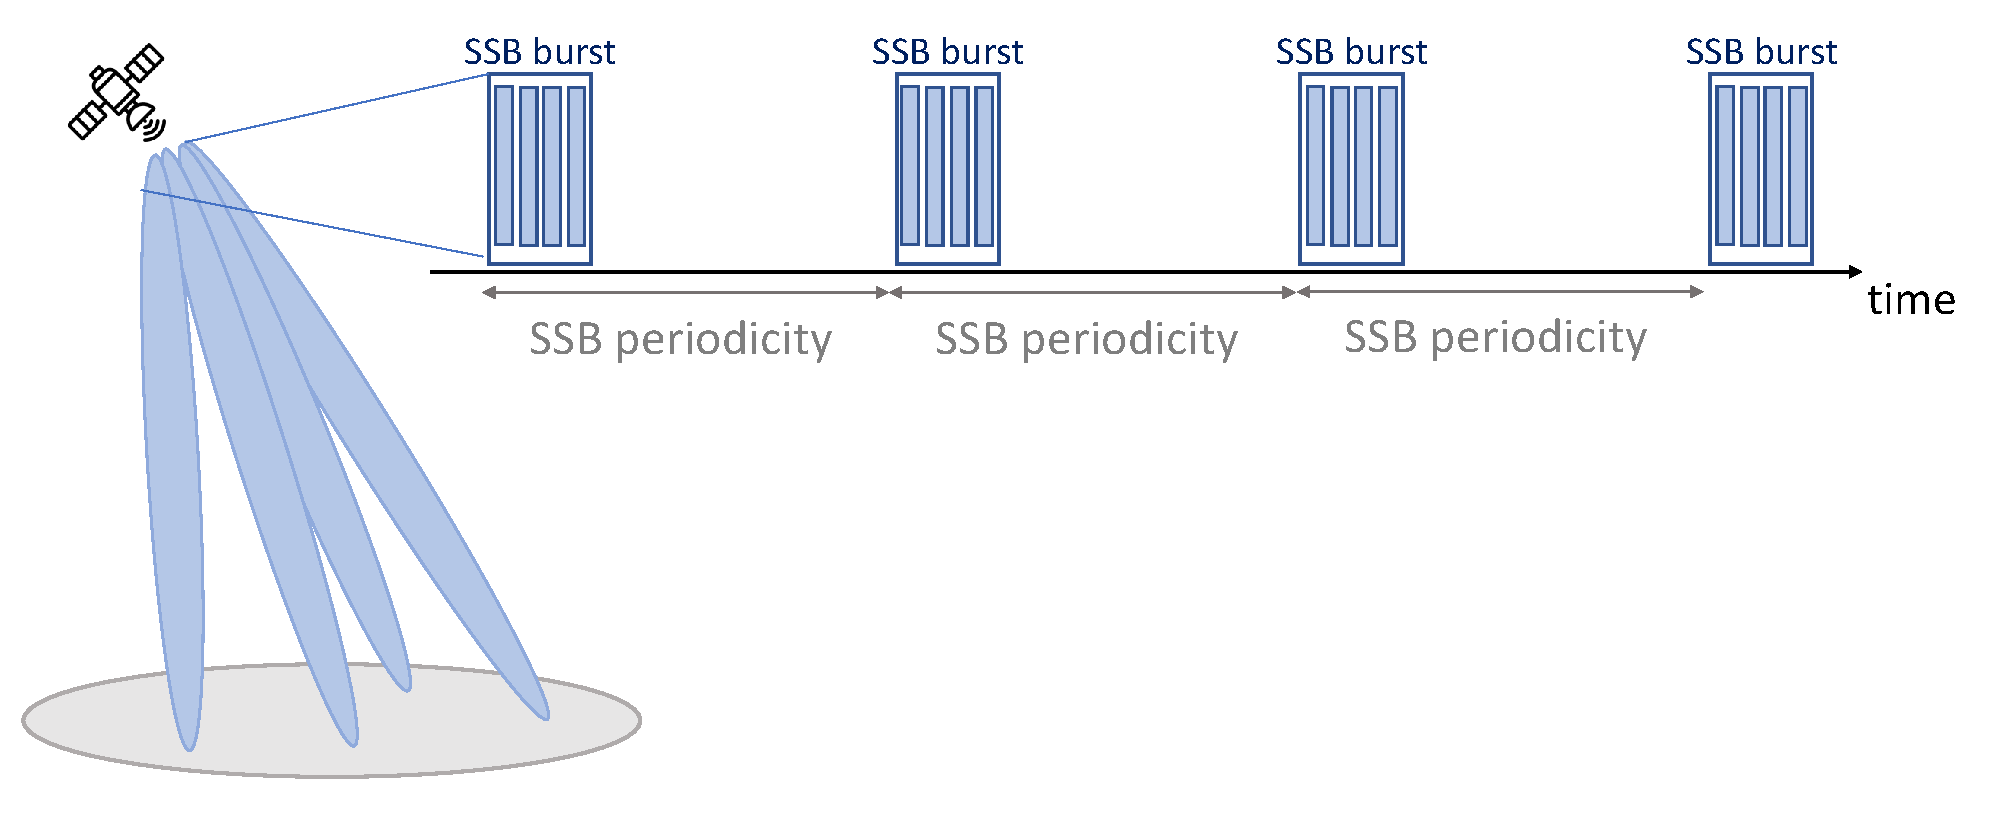
\includegraphics[width=0.8\textwidth]{figure/SSB.pdf}
    \caption{Illustration of SSB configuration.}
    \label{SSB}
\end{figure}

\subsection{SSB in LEO Satellite Network}
In terrestiral network (TN), the base station (gNB) transmits SSBs periodically in time and across different spatial directions through beam sweeping, enabling the UE to detect the best SSB and select the optimal beam for communication. In NTN, the SSBs have the same function but the coverage area of each satellite is much bigger than TN, which means each satellite has to provide service to more cells. Moreover, the long distance from satellite to ground and the power budget of each satellite forces us to properly allocate the power of the SSB. Thus, it is essential for us to manage the SSB transmitted power and the periodicity of each cell.

% The base station (gNB) transmits SSBs periodically in time and across different spatial directions through beam sweeping. Each SSB last for a half frame (5ms). A UE can be provided per serving cell by \emph{ssb-periodicityServingCell}, which is the periodicity of SSB in each serving cell. 

% \subsection{}
% A burst of SSBs covers various directions or beams, enabling the UE to detect the strongest SSB and select the optimal beam for communication. Upon reception, the UE measures the signal quality of the detected SSBs and chooses the best one for initiating the random access procedure.

\section{Related Work}


